%In the following, we 

%\color{blue}




%\revised{:q

In this section, we report on the evaluation process conducted to study the 
performance of \TF. Section~\ref{sec:ResearchQuestions} presents the research 
questions we want to 
answer by means of the performed experiments. 
%the materials and methods used to evaluate \TF. 
%evaluation of \TF, having the {\em goal} of evaluating the performance of the 
%proposed approach. 
Section~\ref{sec:Dataset} 
gives an informative description of the datasets exploited in the evaluation. 
Section~\ref{sec:metrics} and Section~\ref{sec:methodology-metric} describe the 
evaluation metrics and process, respectively. %The experimental results are discussed in the next section. 
To facilitate future research, we made available 
the \TF tool together with the related data in a \GH 
repository.\footnote{\url{https://github.com/ESEM2020-TopFilter/TopFilter}}

%ten equal parts, so-called folds
%We also exploited 
%was also exploited 



\subsection{Research Questions} \label{sec:ResearchQuestions}

%By performing the evaluation, we address 
The following research questions are addressed to study the performance of the proposed approach: %, the:

\begin{itemize}
	\item \rqfirst We investigate different configurations of \TF\ie the 
	number of input topics \emph{t} as well as the number of neighbors \emph{N} 
	is varied, to find the best configuration. %and the considered number of 
	%outcomes \emph{N}.
	
	%\item[--] \rqsecond Because of \TF and \MNB are completely different in 
	%term of input data, we are interested in comparing them by considering 
	%many 
	%factors that can impact on the performance.
	\item \rqsecond  We are interested 
	in understanding if our proposed approach can be used to 
	improve the accuracy of the original \MNB. 
	%From an empirical point of view, it is relevant to analyze the combination 
	%of the two approaches and measure its performances.
\end{itemize}


\subsection{Data Extraction} \label{sec:Dataset}

%\subsection{Data Cleaner}  \label{sec:filter}

%Before encoding topics in the repo-topic ratings matrix, raw topics are pre-processed removing possible syntactical duplicates terms (\eg \textit{document} and \textit{documents}). More specifically, stemming, lemmatization, and stop words removal Natural Language Processing (NLP) techniques have been applied on the mined topics.




%\color{blue}



%The \GH query language \cite{understanding} allows the fetching of relevant repository metadata including name, owner, and list of topics to mention a few. Thus, we \emph{randomly} collected a dataset consisting of 6,258 repositories that use 15,757 topics by means of the GitHub API \cite{pygithub/pygithub_2019}. We employ the \GH star voting mechanism as a popularity measure to avoid including unpopular, unmaintained and toy projects \cite{borges_whats_2018}. As claimed in several works\cite{borges_popularity_2017, borges_predicting_2016}, a high number of stars means the attention of the community for that project. So, we impose the following filter during the query execution:
%\begin{equation}
%\small
%Qf = "is:featured \; topic:t \; stars:100..80000 \; topics:>=2"
%\end{equation}%
%to consider only \GH repositories having a number of stars between 100 and 80,000, and tagged with at least two topics. The boolean qualifier \emph{is:featured} is used in the \MNB work to group repositories given a certain featured topic (please refers to \url{https://github.com/topics} for the complete list of featured topics).

% \cite{MNBreplication}.

To study our proposed approach, we reused the same dataset employed to evaluate 
\MNB and made available by the authors of that technique in a replication 
package.\footnote{\url{https://github.com/MDEGroup/MNB\_TopicRecommendation/}} 
%
%A preprocessing phase was performed to improve the dataset's quality as 
%follows~\cite{repo-topix}. 
%
In particular, to investigate \TF's prediction performances, we populated five 
different datasets starting from the original \MNB corpus by varying the 
\textit{cut-off} value \emph{t}~\cite{10.1145/3383219.3383227}, \ie the 
maximum frequency of the topic distribution (it 
is detailed in Section~\ref{sec:methodology-metric}). In this way, we removed 
infrequent elements from the dataset to analyze their impacts on the overall 
recommendation phase. We firstly filtered the initial set of topics using their 
frequencies counted on the entire \GH dataset. Afterwards, we removed 
irrelevant topics to reduce probable noise during the prediction phase. 
%Through 
%the introduction of the \emph{cut-off} value, we 
%gradually increase the frequency threshold to evaluate possible impacts on 
%overall performances. %, thus we decide to apply it as a first step.
%As \TF is able to retrieve both featured and not-featured topics, such a 
%filtering process does not affect the quality of the collected data.


We developed a filter by means of tailored Python scripts and 
applied it to the initial dataset. As a \GH user can manually specify a topic 
list for a repository, many of them can contain infrequent or improper terms, 
\ie the name 
of the author, duplicated values, or terms that rarely appear, to name a few. 
On one hand, imposing such a preprocessing phase reduces the number of 
repositories to analyze as well as topics to recommend. On the other hand, we 
improve the overall quality of recommendation by removing \emph{``bad''} terms. 
This pruning phase can be done offline and does not affect the time required 
for the recommendation process.



Table \ref{tab:Datasets} summarizes the main features of the datasets, \ie 
$D_1$, $D_5$, $D_{10}$, $D_{15}$, and $D_{20}$, corresponding to different cut-off values \emph{t} = $\{1, 5, 10, 15, 20\}$. \emph{Avg. topics} is the average number of topics that the 
repositories include; \emph{Avg. freq. topics} is the average frequency of the topics in the 
dataset.%, \ie the average occurrences of the topics among  the considered 
%repositories in the dataset.


%\begin{table}[h]
%\centering
%\resizebox{8.5cm}{!} {
%\begin{tabular}{|l|l|l|c|c|}
%\hline
%\textbf{Dataset} & \textbf{No. of repos} &\textbf{ No. of topics} & \textbf{Avg topics for repo} & \textbf{Avg freq. for topic} \\ \hline
%D$_1$  &       6,253      &    15,743       &  9.9  &  3.9       \\ \hline
% D$_5$  &        3,884      &    1,989      &     8.4  &   16.5   \\ \hline
%D$_{10}$  &    2,897         &      964	     &   8.0    &  24.1 \\ \hline
%D$_{15}$  &    2,273        &   634       &   7.8  &  28.1       \\ \hline
%D$_{20}$  &    1,806       &   456        &   7.7 &  30.5       \\ \hline
%
%\end{tabular}
%}
%\caption{Datasets' description.}
%\label{tab:datasets}
%\end{table} 


\begin{table}[h!]
%	\small
	\caption{Datasets.}
	\begin{tabular}{|l|p{0.68cm}|p{0.68cm}|p{0.68cm}|p{0.68cm}|p{0.68cm}|} \hline
		 & $D_{1}$ & $D_{5}$ & $D_{10}$ & $D_{15}$ & $D_{20}$ \\ \hline
		Number of repos & 6,253 & 3,884 & 2,897  & 2,273 & 1,806  \\ \hline
		Number of topics & 15,743 & 1,989 & 964 & 634 & 456 \\ \hline
		Avg. topics & 9.9 & 8.4 & 8.0  & 7.8 & 7.7 \\ \hline
		Avg. freq. topics & 3.9  & 16.5  & 24.1  & 28.1  & 30.5  \\ \hline
	\end{tabular}	
	\label{tab:Datasets}	
\end{table}



\begin{figure*}[t!]
	\centering
	\begin{tabular}{c c }	
		\subfigure[Dataset D$_5$]{\label{fig:dt5_stars}
			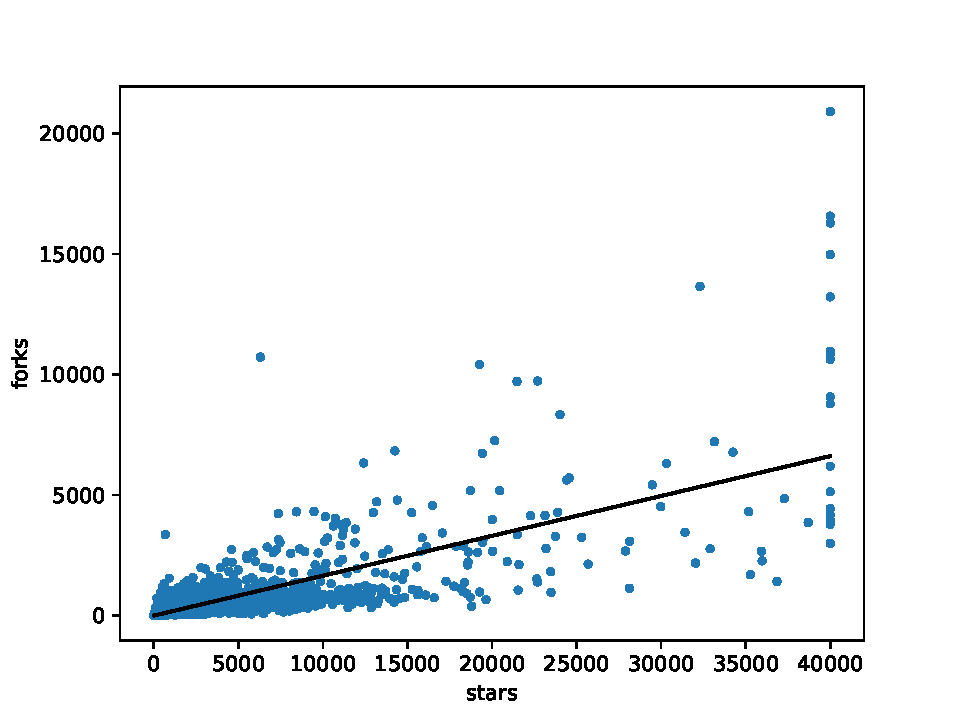
\includegraphics[width=0.45\linewidth]{figs/dataset_5_stars.pdf}} &
		\subfigure[Dataset D$_{10}$]{\label{fig:dt10_stars}
			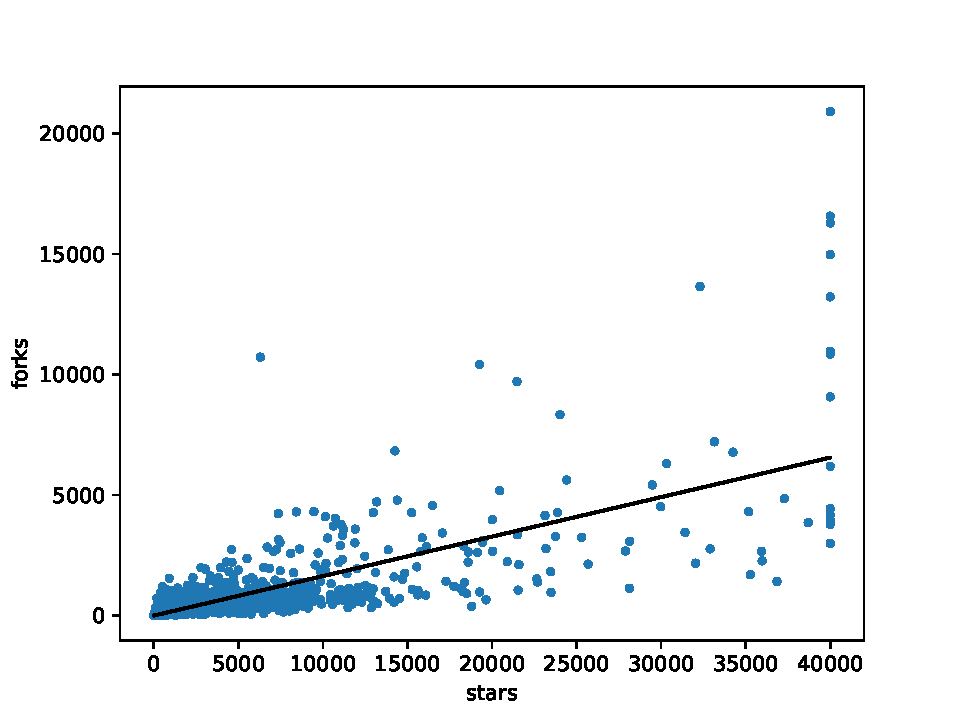
\includegraphics[width=0.45\linewidth]{figs/dataset_10_stars.pdf}} 
			\\
		\subfigure[Dataset D$_{15}$]{\label{fig:dt15_stars}
			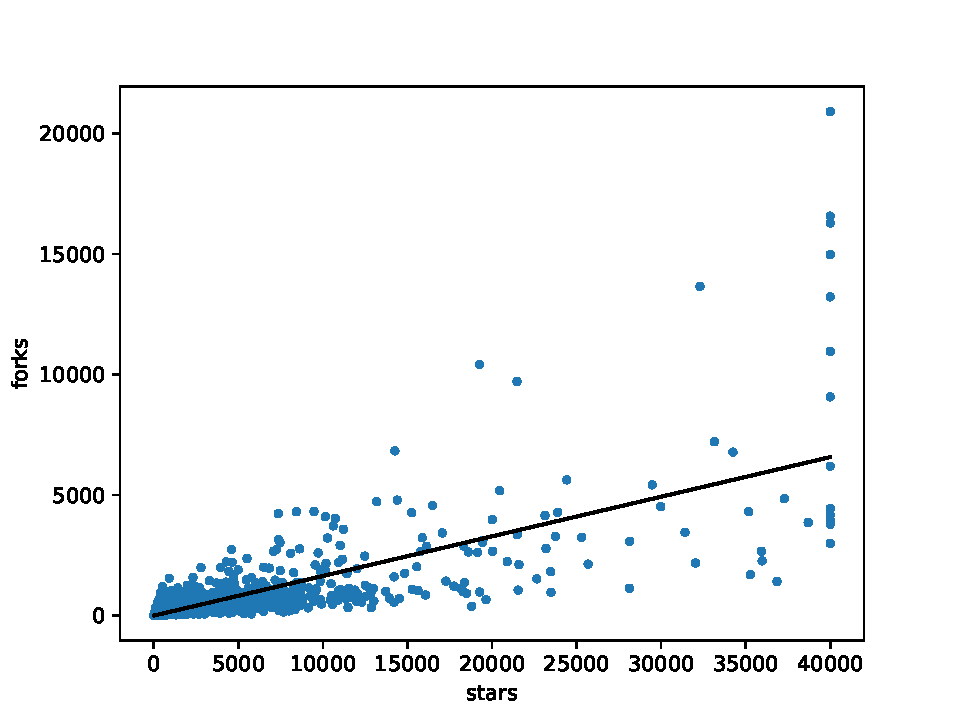
\includegraphics[width=0.45\linewidth]{figs/dataset_15_stars.pdf}} 
			& 	
		\subfigure[Dataset D$_{20}$]{\label{fig:dt20_stars}
			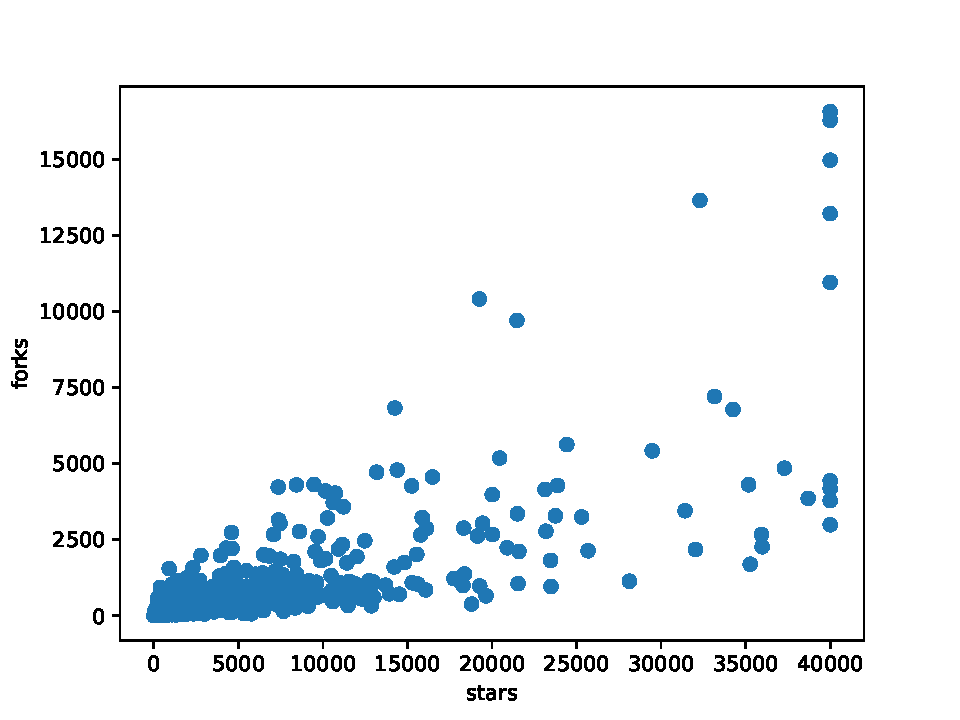
\includegraphics[width=0.45\linewidth]{figs/dataset_20_stars.pdf}}\\
				
	\end{tabular} 
	\caption{A summary of the number of forks and stars for the datasets.} 
	%Quality analysis of the examined datasets
	\label{fig:comparison}
\end{figure*}

%<<<<<<< HEAD
As discussed in Section~\ref{sec:ExperimentalResults}, removing infrequent 
topics improves the overall quality of the considered datasets: %Similarly to 
%the other collaborative filtering approaches, the overall prediction 
%performance strongly depends on the dataset. As we will demonstrate in the 
%next 
%section, 
the collaborative filtering provides better prediction performance when there is enough data, \ie topics in the training set. %to resemble the repository behaviour. 
Once infrequent topics have been removed, all the repositories that contain 
less then five topics are filtered out from the dataset, as they contain little 
information to enable the collaborative filtering prediction. In particular, we 
remove around 2,300 repositories by increasing the cut-off value from 1 to 5. 
It means that the excluded repositories in Dataset D$_5$ are tagged with topics 
that rarely appear in the considered repositories. This finding is strengthened 
by the number of topics, which dramatically decreases to 1,989 when t=5. %The 
%other datasets confirm this trend even though the delta of removed 
%repositories 
%goes down at each filtering step. 
We stop at t=20 and consider Dataset D$_{20}$ as the best one according to our metrics. Additionally, we observe that repositories are tagged by 9.9 and 7.7 topics on average for \emph{t} = 1 and \emph{t} = 20, respectively. This demonstrates that a large number of topics are not beneficial to the discoverability of a project.


 
%=======
%As we can see, removing the infrequent topics improves the overall quality of the considered datasets. In particular, we remove around 2,300 repositories by increasing the cut-off value from 1 to 5. It means that the excluded repositories in Dataset D$_5$ are tagged with topics that rarely appear in the considered repositories. This finding is strengthened by the number of topics, which dramatically decreases to 1,989. The other datasets confirm this trend even though the delta of removed repositories goes down at each filtering step. Thus, we stop at t=20 and consider Dataset D$_{20}$ as the best one according to our metrics. Additionally, we observe that repositories are tagged by 7 topics on average. This demonstrates that a huge number of topics doesn't help the discoverability of a project. 
%>>>>>>> 2241e0e812c956f441252b061dd0d75d6f6927ea

%Furthermore, we evaluate the quality of the OSS project belonging to the examined dataset. As mentioned before, the \GH community assesses this aspect by mainly using forks and stars. 

From the list of projects under analysis, we exploited the \GH API to retrieve 
their number of stars and forks. A summary of the retrieved data is plotted in 
Fig.~\ref{fig:comparison}. %shows the comparison among all the examined 
%datasets. 
Forking is a means to contribute to the original repositories, %~\cite{Jiang:2017:WDF:3042021.3042043}. 
furthermore, there is a strong correlation between forks and stars~\cite{7816479}, as it can be further observed in Fig.~\ref{fig:comparison}. A project with a high number of forks means that it garners attention from the developers community. A repository with a large number of forks can be considered as a well-maintained and well-received project. Whereas, since commits also have an influence on source code~\cite{8009930}, the number of commits is also a good indicator of how a project has been developed. As can be seen, most of the repositories possess a number of stars and forks less than 5,000. A small fraction of them have more than 30,000 forks and 10,000 stars. In this respect, we see that the datasets exhibit a wide variety of quality in terms of the number of forks and stars.
%filtering repositories by the cut-off value \emph{t} helps smooth the distribution. 
%On one hand, 

%Dataset D$_5$ contains more repositories with a high forks number rather than the ultimate dataset, \ie it has around 20,000 forks compared to 15,000 with t=5 and t=20 respectively. On the other hand, the slope depicted in Dataset D$_{20}$ is higher than the original dataset. The positive trend is confirmed by observing the distribution of the other datasets \ie Dataset D$_{10}$ and D$_{15}$. In particular, we are able to remove repositories with less number of stars \ie from 5,000 to 10,000. From this study, we observe a correlation between the number of tars and the topics' frequency. In other words, most frequent topics appear in the high-ranked repositories and this finding affects the quality of the recommendations. 







%Among these projects, only $7$ of them have been forked from other projects. Such original projects have been excluded from the dataset as their forked ones share highly similar libraries, and this may introduce bias in the recommendation outcomes. We represent the distribution of projects with respect to the number of forks, commits and pull requests in Fig.~\ref{fig:ForkCommitPull}. Most projects have a low number of pull requests, \ie lower than 100, however many of them have a large number of forks and commits. Forking is a means to contribute to the original repositories~\cite{Jiang:2017:WDF:3042021.3042043}. Furthermore, there is a strong correlation between forks and stars~\cite{7816479}, as it is further witnessed in Fig.~\ref{fig:ForkStarIssue}. A project with a high number of forks means that it gets attention from the OSS community. In this sense, having many forks can be considered as a sign of a well-maintained and well-received project. Meanwhile, as commits have an impact on the source code~\cite{8009930}, the number of commits is also a good indicator of how a project has been developed.
%}


%e mined dependency specification by means of \code{code.xml} or \code{.grad\-le} files.\footnote{The files \code{pom.xml} and with the extension \code{.gradle} are related to management of dependencies by means of Maven (\url{https://maven.apache.org/}) and Gradle (\url{https://gradle.org/}), respectively.} Fig.~\ref{fig:NumOfLibsD1} depicts the distribution of libraries across the projects. Most of the libraries in \code{D1} ($12,962$) are used by a small number of projects, and only $10$ libraries are extremely popular by being included in more than $200$ projects. By carefully investigating the dataset, we also see that most projects contain a small number of dependencies, \ie $48\%$ of the projects include less than $20$ libraries and just $15\%$ of them include more than $100$ libraries. \}


\subsection{Metrics}\label{sec:metrics}

\begin{figure*}[t!]
	\centering
	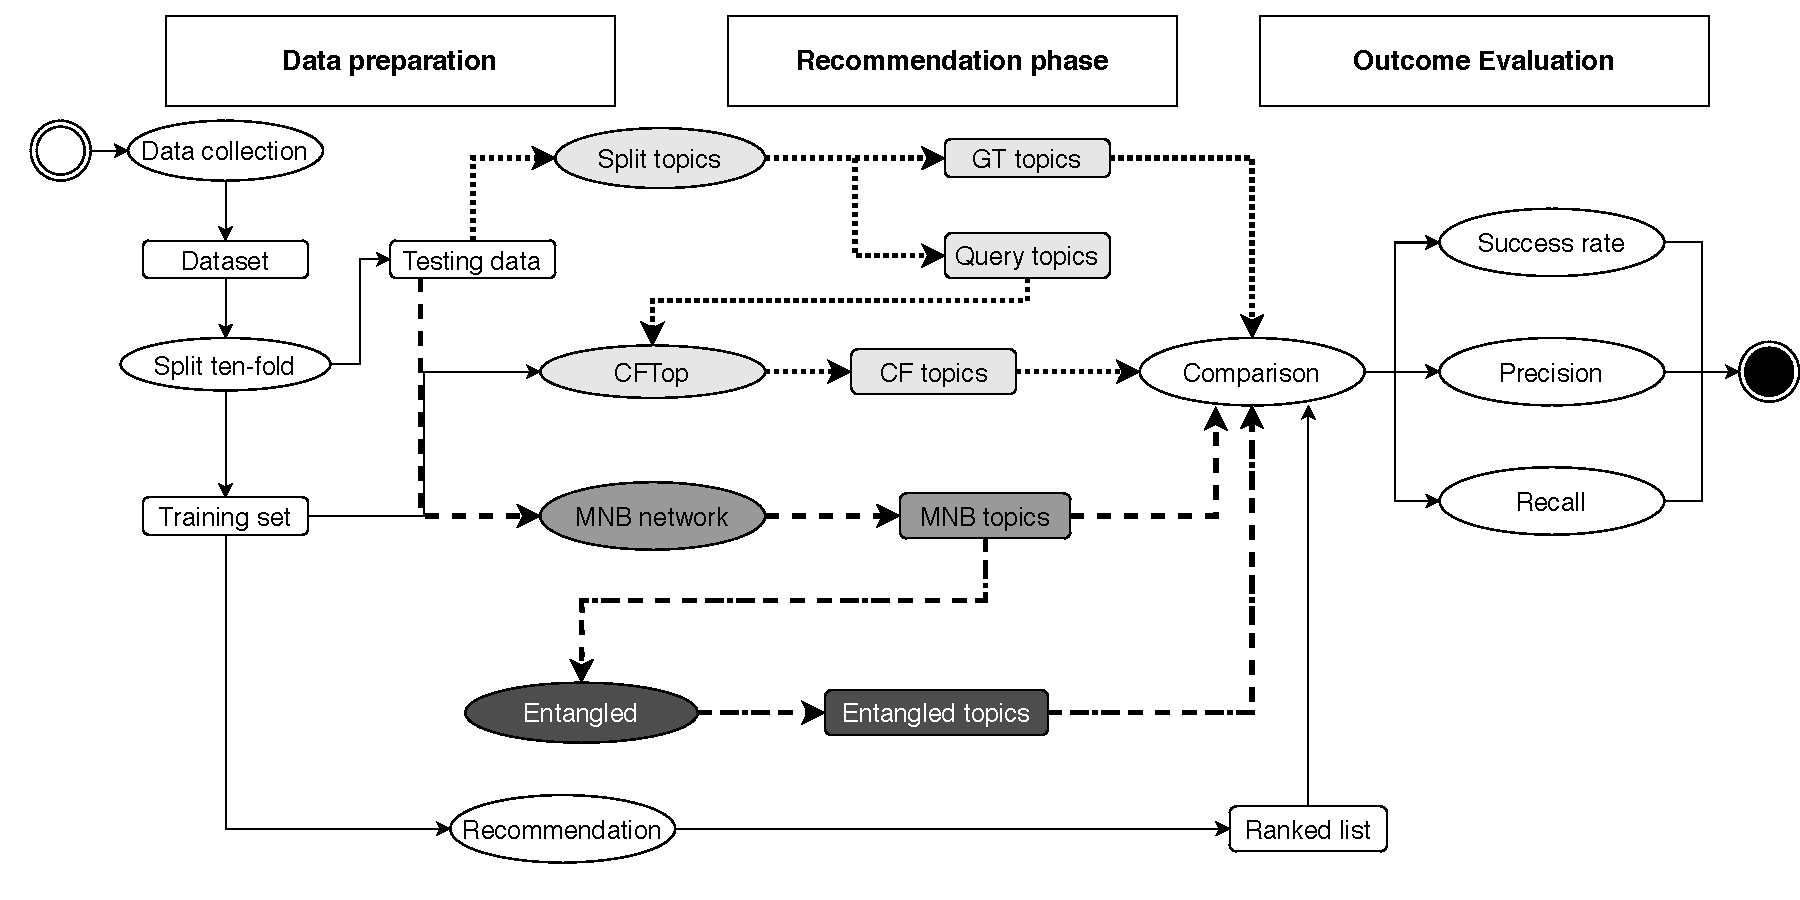
\includegraphics[width=0.96\linewidth,keepaspectratio]{figs/evaluationCF.pdf}
	%\vspace{-.3cm}
	\caption{Evaluation Process.}
	\label{fig:EvaluationProcess}
	\vspace{-.3cm}
\end{figure*}


%In the context of recommendation systems, several metrics have been proposed to evaluate a ranked list of recommended items \cite{DBLP:conf/rweb/NoiaO15}. 
In the scope of this paper, \emph{success rate} \emph{accuracy}, and 
\emph{catalog coverage} are used to study the \TF performance as they have 
been widely exploited by related research~\cite{Robillard:2014:RSS:2631387}. 
% and other studies~\cite{6671293},\cite{Nguyen:2015:ESP:2740908.2742141}.
%Before defining the metrics involved in the experiment, we present the following notations to make easier the understanding of the considered metrics:
First, we introduce the following notations as a base for further presentation:% to make easier the understanding of the metrics involved in our experiment:
\begin{itemize}[noitemsep,topsep=0pt]
	\item \emph{t} is the frequency cut-off value of input topics, \ie all topics that occur less than \emph{t} times are removed from the dataset;
	\item $\tau$ is the number of topics that \TF takes as input;
	\item \emph{N} is the cut-off value for the recommended ranked list of topic;% of recommended libraries;
	\item \emph{k} corresponds to the number of top-similar neighbor projects \TF considers to predict suggested topics;
	\item \emph{GT(p)} is defined as a half of the extracted topics for a testing project \emph{p} using as ground-truth data;%, and \emph{GT(r)} have been used as ground-truth data in the evaluation process;
%	\item For a testing project \emph{r}, a half of its topics are extracted and used as the ground-truth data named as \emph{GT(r)};
	\item $REC_{N}(p)$ is the top-\emph{N}  suggested topics sorted in a descending order;% by considering the recommendation scores;  the outcome of \TF for a given repository \emph{p}, 
	%\item $REC(r)$ is the \emph{top-N} topics recommended to a repository \emph{r}. It is a ranked list in descending order of real scores;
	\item a recommended topic \emph{rt} to a repository \emph{p} is marked as a \emph{match} if $rt \in REC(p)$;
	\item  $match_{N}(p)$ is the set of items in $REC_{N}(p)$ that match with those in \emph{GT(p)} for repository \emph{p}.
\end{itemize}

\noindent By means of the notations, the success rate, accuracy and coverage metrics are defined as follows.  

%\JDR{Rephrase this section}

\vspace{.1cm}
\noindent\textbf{Success rate@N.} Given a set of testing projects \emph{P}, success rate is defined as the ratio of queries that have at least a matched topic among the total number of queries.% In particular, this metric measures the percentage of \emph{top-N} query results that match at least one topic in the \emph{GT(p)} among the number of query project $p \in P$~\cite{6671293}: %It is formally defined as given below:
\vspace{-.1cm}
\begin{equation} \label{eqn:RecallRate}
success\ rate@N=\frac{ count_{p \in P}( \left | match_{N}(p) \right | > 0 ) }{\left | P \right |} %\times 100\%
%success\ rate@N=\frac{ count_{p \in P}( \left | GT(p) \bigcap (\cup_{r=1}^{N} REC_{r}(p)) \right | > 0 ) }{\left | P \right |}
\end{equation}

\vspace{.1cm}
%\vspace{.1cm}
%\noindent \JDR{Check if it will be used} \textbf{Success rate$_M$@N.} Given a set of testing projects \emph{P}, this metric measures the rate at which a recommender system returns at least $M$ topics match among \emph{top-N} items for every project $p \in P$ \cite{6671293}: %It is formally defined as given below:
%\vspace{-.1cm}
%
%\begin{equation} \label{eqn:RecallRate}
%success\ rate_M@N=\frac{ count_{p \in P}( \left | match_{N}(p) \right | >= M ) }{\left | P \right |} %\times 100\%
%%success\ rate@N=\frac{ count_{p \in P}( \left | GT(p) \bigcap (\cup_{r=1}^{N} REC_{r}(p)) \right | > 0 ) }{\left | P \right |}
%\end{equation}
%
%\vspace{.1cm}
%\noindent where the function \emph{count()} counts the number of times that the boolean expression specified in its parameter is \emph{true}.
%Because of \emph{success rate@N} only measures successful queries and it does not reflect how accurate the outcome of a recommender system is (\eg considering two recommendation results where the former counts $1$ topic match out of $5$ and the latter that returns all $5$ topic matches,  both results equally affect the success rate value because they include at least one matched topic), accuracy has been considered as further quality metrics for \TF. 
\noindent \textbf{Accuracy.} Given a list of \emph{top-N} libraries, \emph{precision} and \emph{recall} are utilized to measure the \emph{accuracy} of the recommendation results. In particular,  \emph{precision} is the ratio of the \emph{top-N} recommended topics found in the ground-truth data, whereas \emph{recall} is the ratio of the ground-truth topics belonging to the \emph{N} recommended items \cite{Davis:2006:RPR:1143844.1143874}:%,Nguyen:2019:FRS:3339505.3339636

%However, \emph{success rate@N} does not reflect how accurate the outcome of a recommender system is. For instance, given only one testing project, there is no difference between a system that returns $1$ topic match out of $5$ and another system that returns all $5$ topic matches, since \emph{success rate@5} is $100\%$ for both cases (see Eq.~\eqref{eqn:RecallRate}). Thus, given a list of \emph{top-N} libraries, \emph{precision@N} and \emph{recall@N} are utilized to measure the \emph{accuracy} of the recommendation results. \emph{precision@N} is the ratio of the \emph{top-N} recommended topics belonging to the ground-truth dataset, whereas \emph{recall@N} is the ratio of the ground-truth topics appearing in the \emph{N} recommended items \cite{Nguyen:2019:FRS:3339505.3339636},\cite{DiNoia:2012:LOD:2362499.2362501},\cite{Davis:2006:RPR:1143844.1143874}: %,Nguyen:2015:CRV:2942298.2942305 %}. A concrete definition for the metrics is given below \cite{

%\vspace{-.2cm}
% \cite{Saracevic:1995:EEI:215206.215351}

\begin{equation} \label{eqn:Precision}
precision@N = \frac{ \left | match_{N}(p) \right | }{N}
%precision@N(p) = \frac{\sum_{r=1}^{N}\left | GT(p) \bigcap REC_{r}(p) \right |}{N}
\end{equation}
%\vspace{-.1cm}
\begin{equation} \label{eqn:Recall}
recall@N = \frac{ \left | match_{N}(p) \right | }{\left | GT(p) \right |}
%recall@N(p) = \frac{\sum_{r=1}^{N}\left | GT(p) \bigcap REC_{r}(p) \right |}{\left | GT(p) \right |}
\end{equation}
%\vspace{-.1cm}

\vspace{.1cm}
\vspace{.1cm}



\noindent \textbf{Catalog coverage.} %This metric is particularly suitable to measure the performance predictions of recommendation systems that suggest a list of items \cite{ge_beyond_2010}.
Given the set of projects, we compare the number of recommended topics with the global number of the available ones. %, \ie $ REC_{N}(p)$ and T respectively. 
%Reversely from the previous two metrics, 
This metric measures the suitability of the delivered topics considering all the possible set of values. %From the evaluation point of view, it is interesting to assess the impact of N value on the coverage stability, meaning what values of N impacts on the overall prediction performances. 



\begin{equation}\label{eqn:Coverage}
%coverage = \frac{\left | \cup_{p\in P} \left [  \cup_{r=1}^{N} REC_{r}(p) \right ] \right | }{\left | L \right |} 
coverage@N = \frac{\left | \cup_{p\in P} REC_{N}(p) \right | }{\left | T \right |} 
\end{equation}






\subsection{Evaluation process}\label{sec:methodology-metric}



The \emph{ten-fold cross-validation} technique~\cite{kohavi1995study} has been 
used to assess the performance of \TF and its combined use with \MNB. %and 
%combined approach where every time $9$ folds 
%(each one contains $625$ projects) 
%are used for training and the remaining one for testing.
%
%For each testing project \emph{p}, we randomly deleted a half of its topics 
%and save them as ground-truth data, \emph{GT(p)}, which are then used to 
%validate the recommendation outcomes. The remaining half topics are used as 
%query topics to feed \TF. 
Figure~\ref{fig:EvaluationProcess} depicts the evaluation process consisting of 
three consecutive phases,~\ie~\emph{Data Preparation},~\emph{Recommendation}, 
and~\emph{Outcome Evaluation} and they are going to be explained as follows.

%\noindent
%$\blacksquare$~\textbf{Data Preparation.} 
\vspace{.1cm}
\noindent\textbf{Data Preparation.}
This phase is conducted to collect repositories that match the requirements defined in previous section from GitHub during the \textit{Data collection} step. %The dataset is used to evaluate \TF, \MNB, and the combination of two. 
The dataset is then split into a training and testing set, \ie \code{ Split 
ten-fold}. Due to the different nature of the recommender systems (\ie \MNB 
requires \textit{README} files as input and training data, whereas \TF uses a 
set of assigned topics as input and for training) testing and training 
data needs to be specifically prepared for each approach.
The \code{Split topic} activity resembles a real development process where a developer has already included some topics in the repository, \ie \textit{Query topics} and waits for recommendations. 

%\ie additional topics to be incorporated. \TF recommender system is expected to provide her with the other half, \ie \code{ GT topics}.

%\noindent
%$\blacksquare$~\textbf{Recommendation.} %follows three different flows, according to the required input and produced output of the three mentioned approaches. In particular, the common operations are in white while the three different evaluation flows are represented in a grayscale fashion (\ie light grey, grey and dark grey boxes are related to \TF, \MNB, and \code{Entangled} approaches evaluation respectively). 
\vspace{.1cm}
\noindent\textbf{Recommendation.} To enable the evaluation of \TF, we extracted a portion of topics from a given testing project, \ie the ground-truth part. The remaining part is used as a query to produce recommendations. %(see the dotted line flow).
Since \MNB uses only README file(s) to predict a set of topics, it does not require any topics as input. The approach parses and encodes text files in vectors using the TF-IDF weighting scheme. 
%To feed the network that delivers a set of topics (see the bold line). 
Finally, the combined approach uses \TF as the recommendation engine which is fed by topics generated by \MNB. In this respect, both \textit{Testing data} and \textit{Training set} boxes are simplified to provide the needed data, \ie README files and assigned topics to the recommender systems.

%\noindent
%$\blacksquare$~\textbf{Outcome Evaluation.} 
\vspace{.1cm}
\noindent\textbf{Outcome Evaluation.} It is worth noting that we cannot 
directly compare \TF with \MNB since they 
rely on different input data. To be concrete, \TF is a supervised learning 
system that requires an initial set of assigned topics for the training, 
whereas \MNB is unsupervised learning and it uses only information mined from 
README files to recommend, without making use of any topics as input. Thus, we 
evaluate the performance of \TF by analysing the recommendation results that 
are compared with those stored as ground-truth data to compute the quality 
metrics (\ie \textit{Success rate}, \textit{Precision}, \textit{Recall}, and 
\textit{Catalog coverage}) during the \textit{RQ$_1$} evaluation activities. 
The same metrics are used to evaluate the performance of the combined use of 
\TF and \MNB to answer \textit{RQ$_2$}.

%In this stage, recommendation results are compared with those stored as 
%ground-truth data to compute the quality metrics, \ie \textit{Success rate}, 
%\textit{Precision}, \textit{Recall}, and \textit{Catalog coverage}) during the 
%\textit{RQ$_1$} and \textit{RQ$_2$} evaluation activities.  

%, which are called \emph{\textbf{te}}, and serve as input for \code{Similarity Computation} and \code{Recommendation} components.


%
%\subsection{Research Questions} \label{sec:ResearchQuestions}
%
%%By performing the evaluation, we address
%The following research questions are addressed to study the performance of the 
%proposed approaches:
%
%\begin{itemize}
%	\item \rqfirst We investigate different configurations of \TF\ie the 
%	number of input topics \emph{t} as well as the number of neighbors \emph{N} 
%	is varied, to find the best configuration. %and the considered number of 
%	%outcomes \emph{N}.
%	
%	%\item[--] \rqsecond Because of \TF and \MNB are completely different in 
%	%term of input data, we are interested in comparing them by considering 
%	%many 
%	%factors that can impact on the performance.
%	\item \rqsecond \TFb is an extended version of \MNB, thus we are interested 
%	in understanding if our proposed approach outperforms the original \MNB. 
%	%From an empirical point of view, it is relevant to analyze the combination 
%	%of the two approaches and measure its performances.
%\end{itemize}
%



%To assess the performance of \CR proposed approach, we applied ten-fold cross-validation, considering every time $9$ folds (each one contains $625$ projects) for training and the remaining one for testing. 
%	For every testing project \emph{p}, a half of its topics are \emph{randomly} 
%	taken out and saved as ground truth data, let us call them \emph{GT(p)}, which will be used to validate the recommendation outcomes. The other half are used 
%	as testing libraries or query, which are called \emph{\textbf{te}}, and serve 
%	as input for \code{Similarity Computation} and \code{Recommendation}.
%The splitting mimics a real development process where a 
%developer has already included some topics in the current project, \ie 
%\emph{\textbf{te}} and waits for recommendations, that means additional topics to be incorporated. A recommender system is expected to provide her 
%with the other half, \ie \emph{GT(p)}. %To ensure a reliable comparison between \LR and \CR, we performed cross-validation for both using exactly the same folds.
%
%
%
%There are several metrics available to evaluate a ranked list of recommended items \cite{DBLP:conf/rweb/NoiaO15}. In the scope of this paper, \emph{success rate}, \emph{accuracy}, \emph{sales diversity}, and \emph{novelty} have been used to study the systems' performance as already proposed by Robillard \etal~\cite{Robillard:2014:RSS:2631387} and other studies~\cite{6671293},\cite{Nguyen:2015:ESP:2740908.2742141}. For a clear presentation of the metrics considered during the outcome evaluation, let us introduce the following notations:
%
%\begin{itemize}[noitemsep,topsep=0pt]
%	\item \emph{N} is the cut-off value for the ranked list;% of recommended libraries;
%	\item \emph{k} is the number of neighbor projects exploited for the recommendation process;
%	\item For a testing project \emph{p}, a half of its libraries are extracted and used as the ground-truth data named as \emph{GT(p)};
%	\item $REC(p)$ is the \emph{top-N} libraries recommended to \emph{p}. It is a ranked list in descending order of real scores;%, with $REC_r(p)$ being the recommended library in the position $r$.		
%	\item If a recommended library $l \in REC(p)$ for a testing project $p$ is found in the ground truth of $p$ (\ie \emph{GT(p)}), hereafter we call this as a library \textit{match} or \textit{hit}.	
%\end{itemize}	
%
%
%
%If $REC_{N}(p)$ is the set of top-$N$ items and $match_{N}(p)=  GT(p) \bigcap REC_{N}(p) $ is the set of items in the \emph{top-N} list that match with those in the ground-truth data, then the metrics are defined as follows.
%
%\paragraph{\textbf{Success rate@N}} Given a set of testing projects \emph{P}, this metric measures the rate at which a recommender system returns at least a topic match among \emph{top-N} items for every project $p \in P$ \cite{6671293}: %It is formally defined as given below:
%\vspace{-.3cm}
%
%\begin{equation} \label{eqn:RecallRate}
%success\ rate@N=\frac{ count_{p \in P}( \left |  match_{N}(p) \right | > 0 ) }{\left | P \right |} %\times 100\%
%%success\ rate@N=\frac{ count_{p \in P}( \left |  GT(p) \bigcap (\cup_{r=1}^{N} REC_{r}(p)) \right | > 0 ) }{\left | P \right |} 
%\end{equation}
%
%\noindent where the function \emph{count()} counts the number of times that the boolean expression specified in its parameter is \emph{true}.
%
%
%\paragraph{\textbf{Accuracy}} Accuracy is considered as one of the most preferred \emph{quality indicators} for Information Retrieval applications \cite{Saracevic:1995:EEI:215206.215351}. However, \emph{success rate@N} does not reflect how accurate the outcome of a recommender system is. For instance, given only one testing project, there is no difference between a system that returns $1$ topic match out of $5$ and another system that returns all $5$ topic matches, since \emph{success rate@5} is $100\%$ for both cases (see Eq.~\eqref{eqn:RecallRate}). Thus, given a list of \emph{top-N} libraries, \emph{precision@N} and \emph{recall@N} are utilized to measure the \emph{accuracy} of the recommendation results. \emph{precision@N} is the ratio of the \emph{top-N} recommended topics belonging to the ground-truth dataset, whereas \emph{recall@N} is the ratio of the ground-truth topics appearing in the \emph{N} recommended items \cite{Nguyen:2019:FRS:3339505.3339636},\cite{DiNoia:2012:LOD:2362499.2362501},\cite{Davis:2006:RPR:1143844.1143874}: %,Nguyen:2015:CRV:2942298.2942305 %}. A concrete definition for the metrics is given below \cite{
%
%%\vspace{-.2cm}
%% \cite{Saracevic:1995:EEI:215206.215351}
%
%\begin{equation} \label{eqn:Precision}
%precision@N = \frac{ \left |  match_{N}(p) \right | }{N}
%%precision@N(p) = \frac{\sum_{r=1}^{N}\left |  GT(p) \bigcap REC_{r}(p) \right |}{N}
%\end{equation}
%%\vspace{-.1cm}
%\begin{equation} \label{eqn:Recall}
%recall@N = \frac{ \left |  match_{N}(p) \right | }{\left | GT(p) \right |}	
%%recall@N(p) = \frac{\sum_{r=1}^{N}\left |  GT(p) \bigcap REC_{r}(p) \right |}{\left | GT(p) \right |}	
%\end{equation}
%%\vspace{-.1cm}
%






